\documentclass[a4paper,UTF8]{article}
\usepackage{ctex}
\usepackage[margin=1.25in]{geometry}
\usepackage{color}
\usepackage{graphicx}
\usepackage{amssymb}
\usepackage{amsmath}
\usepackage{amsthm}
\usepackage{soul, color, xcolor}
\usepackage{bm}
\usepackage{tcolorbox}
\usepackage{hyperref}
\numberwithin{equation}{section}
%\usepackage[thmmarks, amsmath, thref]{ntheorem}
\theoremstyle{definition}
\newtheorem*{solution}{Solution}
\newtheorem*{prove}{Proof}
\usepackage{multirow}
\usepackage{diagbox}
\usepackage{float}

% \begin{figure}[H]
%	\centering
%	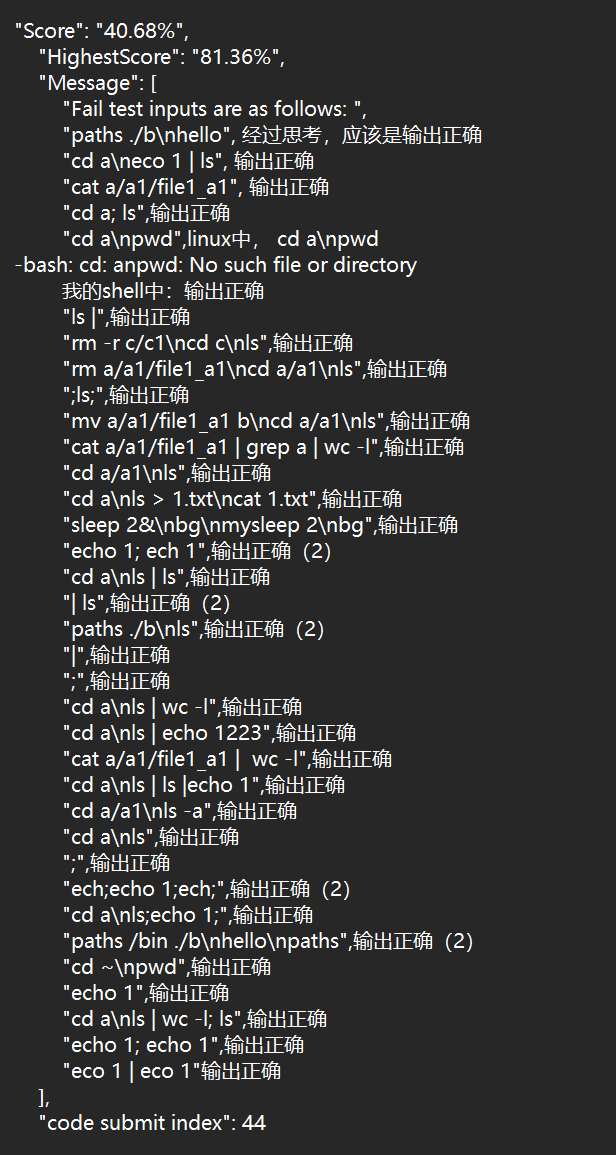
\includegraphics[width=1\textwidth]{1.png}\\
%	\caption{local test}
%	\label{fig:local test}
% \end{figure}  

\begin{document}
\title{Life-parallel 实验报告}
\author{221300079, 王俊童, \href{mailto:221300079@smail.nju.edu.cn}{221300079@smail.nju.edu.cn}}
\maketitle

    

    \section{设计方案}

    讲一下我的设计思路吧。

    一开始本来没看到那个创建函数是不能用超过threads次的,所以打算每次创建之后销毁就可以了。但是后来看见了这个开始思考如何才能够存放线程呢?
    于是就想到了线程池这个东西。

    但是我一开始拿线程池做的并不顺利,因为我想的是既然create函数就执行一次func,那么我就用这个execute函数多去执行几次就好了,事实上,这样就不算是并行了
    所以这个oj不接受我的代码,尽管我跑的很快。(某种意义上说为啥这个不算呢,反正就是速度达到了相当快的地步...)

    后来我又咨询了一下其他同学的意见,再此处感谢人工智能学院 221300004 王晨阳同学对于我的帮助,我跟他进行了一些关于线程池的讨论和开拓,最后各自确定了一套方案并加以完成。

    所以并发这个东西还是很麻烦的,但是不知道为什么最后难点全部到处理函数的速度上面去了...
    
    \section{其余问题}

    无。

\end{document}